% Template for ICIP-2013 paper; to be used with:
%          spconf.sty  - ICASSP/ICIP LaTeX style file, and
%          IEEEbib.bst - IEEE bibliography style file.
% --------------------------------------------------------------------------
\documentclass{article}
\usepackage{spconf,amsmath,graphicx}
\usepackage[frenchb]{babel}
\usepackage[utf8]{inputenc}
\usepackage{graphicx}
\usepackage{subcaption}


% Title.
% ------
\title{D\'{E}CONVOLUTION D'IMAGES FLOUES PAR FILTRAGE CLS}
%
% Single address.
% ---------------
%\name{Author(s) Name(s)\thanks{Thanks to XYZ agency for funding.}}
%\address{Author Affiliation(s)}
%


\name{\qquad Julien Guichon \qquad Dimitri Gominski \qquad \qquad}

\address{}
	
\begin{document}
%\ninept
%
\maketitle
%
\begin{abstract}
	
	Image deblurring is a famous inverse problem in image processing, and can be frustrating because of the lack of information to retrieve the original image, often noisy and/or blurred with complex camera motion. It implies that the solution has to make assumptions on the acquisition system or the original image, and has to be robust against the heavy impact noise can have through the treatment.
	
	This reports study the performance and the limitations of the Constrained Least Squares (CLS ) approach. We also compare it to other famous algorithm, in order to determine under which conditions it should be use.
	
\end{abstract}
%

%
\section{Introduction}
\label{sec:intro}

	Le traitement de défloutage revient en termes mathématiques à effectuer une déconvolution sur l'image floutée. En effet, si $f(x,y)$ désigne l'image d'entrée, un "floutage" linéaire et indépendant de la position est modélisé par une opération de convolution par un noyau $h(x,y)$ qui donne l'image floutée $g(x,y)$ :
	$$g(x,y) = f(x,y) \otimes h(x,y)$$ 
	
	Dans ce cas, l'opération rigoureusement inverse de la convolution (déconvolution), correspondant à la résolution d'un système d'équations, suffit à retrouver exactement l'image de départ.
	
	Mais l'image d'entrée présentant systématiquement un bruit dû à l'acquisition, et les traitements numériques étant intrinsèquement sources de bruit, nous devons considérer un bruit additif n(x,y) : 
	$$g(x,y) = f(x,y) \otimes h(x,y) + n(x,y)$$ 
	
	Et c'est ce bruit qui complique grandement les calculs, puisque l'opération de déconvolution va l'amplifier au point de rendre l'image de sortie complètement inutilisable [2].
	
	Pour simplifier les notations et calculs, passons en calcul matriciel dans le domaine fréquentiel : 
	$$G = F * H + N$$
	
	Il existe 2 familles d'algorithmes de défloutage : les algorithmes qui supposent le noyau de floutage connu ($H$), et les algorithmes "à l'aveugle" où aucune supposition n'est faite sur le processus de floutage.
	
	

\section{Floutages usuels}

	Le floutage peut être dû : 
	\begin{itemize}
	\item à des mouvements intempestifs du système d'acquisition ou de l'objet lors de la prise
	\item à des perturbations optiques lors du passage des rayons lumineux dans certains milieux (verre, eau)
	\item à une modification de la distance focale pendant la prise (zoom/dézoom, parfois voulu)
	\end{itemize}

	On caractérise ce floutage par un noyau $h(x,y)$. Cette fonction qu'on appelle PSF (\textit{Point Spread Function}) donne la réponse d'un théorique "système de floutage" (système qui donnerait l'image de sortie floutée à partir de l'image d'entrée) à une entrée correspondant à un point lumineux au centre de l'image (impulsion lumineuse). Son équivalent fréquentiel est appelé OTF (\textit{Optical Transfer Function}). Ci-dessous deux exemples de noyaux usuels :
	
	\begin{figure}[h]
		\begin{center}			
			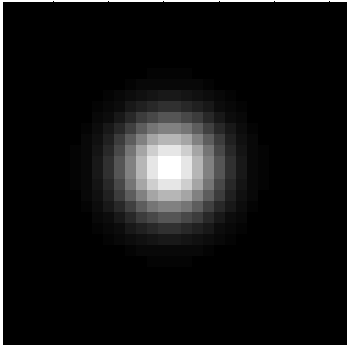
\includegraphics[scale=0.3]{Img/blurkernel_gauss}
		\end{center}
		\caption{Noyau de floutage gaussien}
	\end{figure}

	
	\begin{figure}[h]
	\begin{center}			
		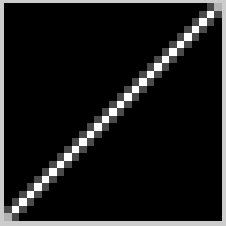
\includegraphics[scale=0.48]{Img/blurkernel_linear}
	\end{center}
	\caption{Noyau de floutage linéaire}
	\end{figure}

	Le noyau linéaire correspond par exemple à un mouvement linéaire de l'appareil pendant la prise, et le noyau gaussien à une capture à travers du verre (diffusion).
	Ces exemples étant très courants, nous ferons notre étude de l'algorithme CLS sur ces deux noyaux.
	

\section{Approches classiques - bibliographie}

	Plusieurs méthodes ont été proposées pour trouver une estimation correcte $\hat f$ de l'image d'origine $f$ à partir de la sortie $g$, en supposant le noyau de floutage $h$ connu.
	
	De manière générale, l'idée pour pouvoir effectuer une déconvolution en limitant les effets du bruit est de le filtrer aux fréquences concernées. Aux fréquences non impactées par le bruit, l'opération dans le domaine fréquentiel doit idéalement être une inversion, en effet si $N(f_1,f_2) = 0$, on a $G(f_1,f_2) = \hat F(f_1,f_2) * H(f_1,f_2)$ donc :
	$$\hat F(f_1,f_2) = G(f_1,f_2) * H^{-1}(f_1,f_2)$$
	
	Application du filtre de Wiener qui fait usage de la répartition spectrale du signal et du bruit supposées connues, la déconvolution de Wiener [4] propose une estimation $\hat F$ comme suit :
	$$\hat F = \frac {1}{H} \bigg[ \frac {|H|^2}{|H|^2 + \frac {|N|^2}{|F|^2} } \bigg] * G$$
	
	On voit que le filtre appliqué à G est lié à l'évolution du rapport signal/bruit $\frac{|F|^2}{|N|^2}$ dans le domaine fréquentiel, de manière à ce que les fréquences polluées ($\frac{1}{SNR} { \rightarrow +\infty}$) soient éliminées avec l'augmentation du dénominateur, tandis qu'aux fréquences non polluées ($\frac{1}{SNR} { \rightarrow 0}$) on fasse rigoureusement une inversion de $H$.
	
	Cette opération revient à minimiser l'erreur quadratique moyenne entre l'image d'entrée et son estimation, son défaut est de faire des hypothèses fortes sur le bruit et l'image d'entrée qui ne sont pas toujours disponibles.
	\\
	
	Les papiers [5] et [6] proposent de décomposer la matrice $H$, de manière à fournir des coefficients caractéristiques sur lesquels on peut agir pour réduire les effets du bruit, notamment avec la décomposition SVD qui fournit la décomposition suivante d'une matrice M :
	$$ M = U \Sigma V^*$$
	
	Avec $\Sigma$ matrice diagonale des coefficients. Une telle décomposition facilite la résolution du problème inverse du floutage, mais se révèle très conséquente en temps de calcul.
	\\
	
	Des approches statistiques [7] ont également été essayées, où une première estimation du noyau de floutage est donnée puis affinée au cours de plusieurs itérations, selon un critère de vraisemblance à minimiser.
	
	Plus rapides, ces méthodes permettent également de traiter les images floutées selon des noyaux complexes.
	\newpage
	
	
\section{Approche Constrained Least Squares}

	Très similaire au filtre de Wiener, la méthode Constrained Least Squares, sous la contrainte $||G - H \hat{F}||^2 = ||N||^2$, vise à minimiser la quantité :
	$$\sum\limits_{i=0}^{M-1} \sum\limits_{i=0}^{N-1} \big[\nabla ^2 f(x,y)]^2 $$
	
	Cette quantité traduisant l'homogénéité ("smoothness") de l'image. Cela revient à minimiser la fonction d'erreur :
	$$||g - h \otimes \hat{f}||^2 _2 + \gamma ||\Delta \hat{f}||^2 _2$$
	
	Il n'y a ici pas de présupposé sur l'image de départ.
	En domaine fréquentiel la solution prend la forme :
	$$\hat F = \frac {1}{H} \bigg[ \frac {|H|^2}{|H|^2 + \gamma |P|^2 } \bigg] * G$$ 
	
	où P est l'opérateur laplacien en domaine fréquentiel : 
	$$ P = DFT\bigg\{\begin{bmatrix}
		0 & -1 & 0 \\
		-1 & 4 & -1 \\
		0 & -1 & 0 
		\end{bmatrix}\bigg\}$$
		
	et $\gamma$ est un paramètre à ajuster pour satisfaire la contrainte.
	\\
	
	Notons que l'opérateur Laplacien en domaine fréquentiel possède une amplitude forte pour les fréquences élevées (d'où son utilisation en détection de contour). Dans le cas présent, se trouvant au dénominateur, il aura tendance à \textit{diminuer} l'effet des hautes fréquences, où se trouve généralement le bruit, tandis qu'en basses fréquences on aura comme pour le filtre de Wiener une inversion simple de $H$.
	
	$\gamma$ permet d'ajuster un compromis entre le bruit et la précision du défloutage. Son réglage peut se faire à l'aveugle selon le résultat voulu, ou par calcul en satisfaisant la contrainte sus-citée. 


\section{Contexte d'application}

	Nous implémentons cet algorithme CLS en langage C++, en proposant une interface graphique pour importer des images, choisir le noyau de floutage à considérer pour la déconvolution (linéaire/gaussien) et les paramètres associés (angle, longueur pour le linéaire, taille et sigma pour le gaussien), et visualiser les résultats.
	
	Le traitement repose sur la bibliothèque OpenCV (licence libre), qui propose des méthodes pour la manipulation de fichiers d'image et les opérations de base pour le traitement d'image.

\section{Application et résultats}

	Ci-dessus une démonstration des résultats de l'algorithme CLS sur une situation correspondant à un floutage linéaire, avec présence de bruit.
	
	\begin{figure}[!h]
		\begin{center}			
			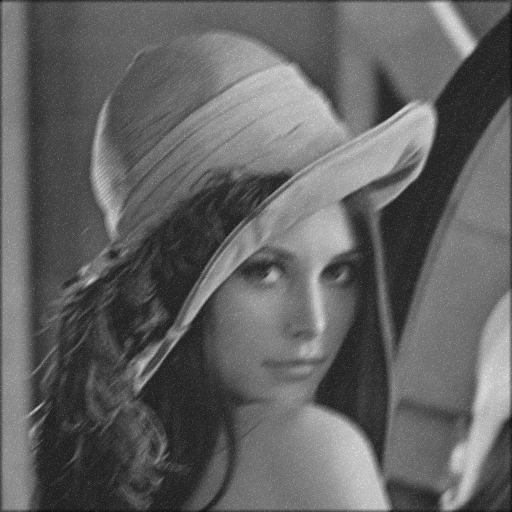
\includegraphics[scale=0.3]{Img/MLbefore}
		\end{center}
		\caption{Floutage linéaire d'angle 45, longueur 10}
	\end{figure}

	\begin{figure}[!h]
	\begin{center}			
		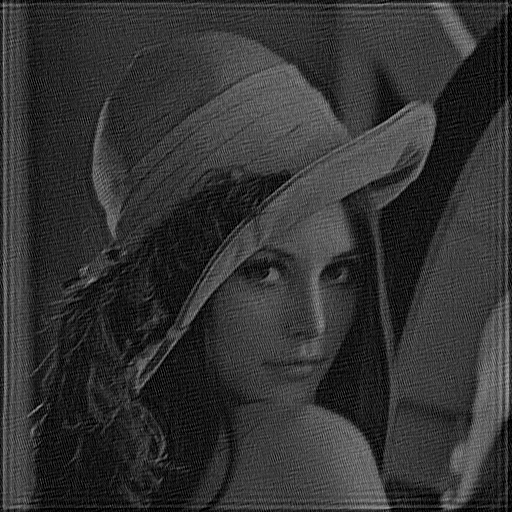
\includegraphics[scale=0.3]{Img/MLafterg001}
	\end{center}
	\caption{Résultat après traitement CLS, $\gamma = 0.01$}
	\end{figure}

	\begin{figure}[!h]
	\begin{center}			
		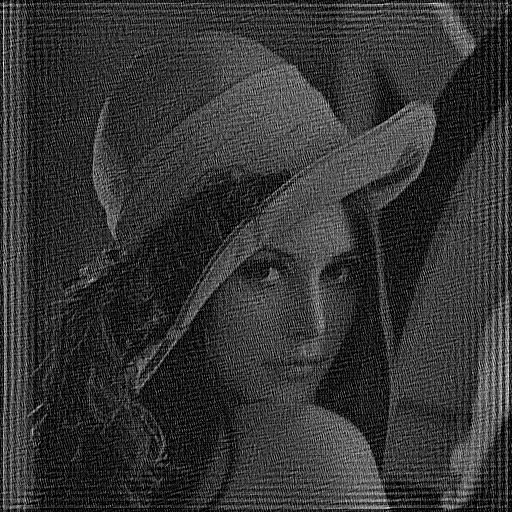
\includegraphics[scale=0.3]{Img/MLafterg0001}
	\end{center}
	\caption{Résultat après traitement CLS, $\gamma = 0.001$}
	\end{figure}

	Deux phénomènes sont mis en évidence :
	\begin{itemize}
		\item l'image traitée perd en luminosité
		\item l'évolution de $\gamma$ met en évidence le compromis bruit/défloutage\\ 
	\end{itemize}
	
	Dans cet exemple, $\gamma = 0.01$ semble être le meilleur compromis.
	\newpage
	
	Pour caractériser les performances de l'algorithme CLS, ci-dessous un tableau regroupant l'erreur quadratique moyenne (MSE, Mean Square Error) par rapport à l'image nette sur diverses situations, avec diverses valeurs de gamma.
	
	\begin{figure}[!h]
		\begin{center}			
			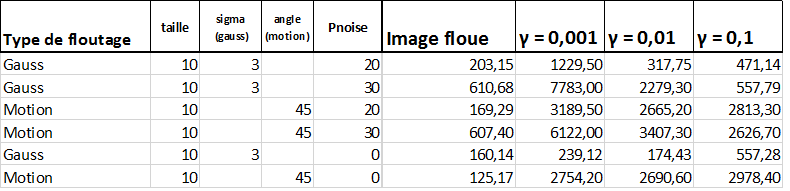
\includegraphics[scale=0.4]{Img/tabmse}
		\end{center}
		\caption{Batterie de tests, mesure de la MSE}
	\end{figure}
	
	Idem pour le PSNR (Peak Signal to Noise Ratio), qui estime le rapport signal/bruit :
	
	\begin{figure}[!h]
		\begin{center}			
			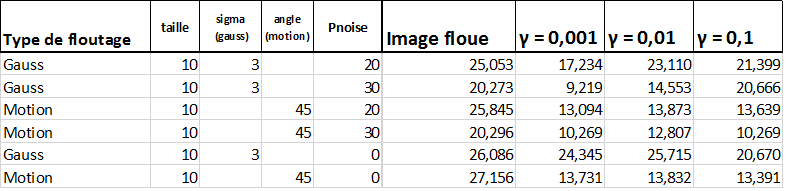
\includegraphics[scale=0.4]{Img/tabpsnr}
		\end{center}
		\caption{Batterie de tests, mesure du PSNR}
	\end{figure}


	Nous n'obtenons qu'un seul cas d'amélioration au sens de la MSE et du PSNR, dans le cas du floutage gaussien très bruité (taille 10, $\sigma = 3$, puissance du bruit : 30 dbW) pour $\gamma = 0.1$.
	Pour exemple, ci-dessous le cas du défloutage du mouvement linéaire (taille 10, angle 45\degre, puissance du bruit : 30 dbW), $\gamma = 0.001$, où l'image produite devient illisible. Cela montre les limites de l'algorithme qui peut également dégrader l'image de départ.
	
	\begin{figure}[!h]
		\begin{center}			
			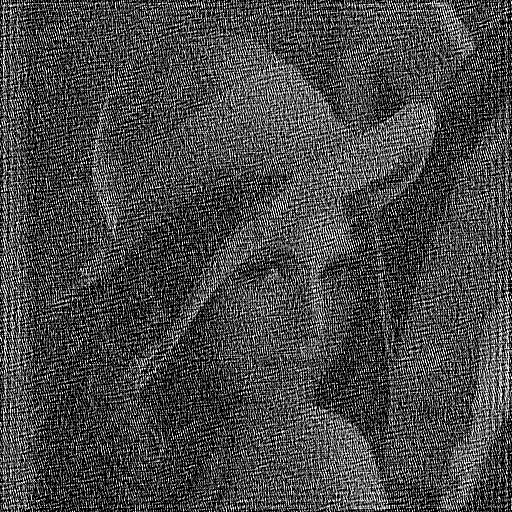
\includegraphics[scale=0.4]{Img/echec}
		\end{center}
		\caption{Exemple d'image dégradée}
	\end{figure}
	
	Une première constatation s'impose : on arrive très difficilement à améliorer la MSE et le PSNR avec ce traitement de défloutage, et dans le cas du floutage par mouvement linéaire les résultats sont mauvais. Il est important de souligner que ces mesures ne permettent pas de traduire précisément la "netteté" de l'image qui est en soi l'objectif de ce traitement : elles ne mesurent qu'un écart entre l'image traitée et l'image d'origine. Néanmoins, leur évolution lors du réglage de $\gamma$ aide à choisir une valeur optimale.
	
	Deuxième conclusion : $\gamma$ influence fortement la qualité de l'image de sortie, et son bon réglage semble essentiel pour optimiser le résultat. Nous avons obtenu les meilleurs résultats pour des valeurs entre 0.01 et 0.1, au delà les effets dûs à l'amplification du bruit ou le flou deviennent prédominants.
	
	
\section{Critique et domaine d'utilisation}

	De par ses hypothèses faibles et sa simplicité de calcul, le filtrage CLS nous semble être intéressant pour les traitements de défloutage simples (mouvement linéaire, flou gaussien), même lorsque le noyau n'est pas connu précisément puisqu'on peut alors simplement procéder par itération. 
	
	Un algorithme d'optimisation de $\gamma$ pourra sans doute produire des résultats plus précis, cependant à notre sens si l'objectif est de produire des images plus nettes par exemple pour permettre de déchiffrer du texte, cette précaution n'est pas nécessaire puisqu'on obtient des résultats satisfaisant en procédant à l'aveugle (et nous préconisons de commencer avec $\gamma = 0.01$).
	
	Les cas où le filtrage CLS devient insuffisant sont les cas de floutage complexe (mouvement non linéaire par exemple), les cas où le floutage dépend de la position sur l'image (limite intrinsèque) et les cas où le bruit est trop complexe/fort pour permettre une approche classique de filtrage haute fréquence.
	
	
\section{Conclusion}

	L'algorithme de déconvolution par approche Constrained Least Squares, de par son implémentation rapide et ses résultats satisfaisants dans des cas simples de floutage, nous semble être un outil essentiel dans la panoplie des méthodes de restauration d'image.

\nocite{*} 
\bibliographystyle{plain}
\bibliography{strings}



\end{document}
